\documentclass[5p]{elsarticle} % seleccionar: preprint, review, 1p, 3p, 5p



\usepackage{mathtools}
\journal{ }


%to force all images and table in one single section
\usepackage{placeins}
% It is necesary to add \FloatBarrier in the text. 
% After that order, all the floating are shown.

%%%%%%%%%%%%%%%%%%%%%%%
%% Elsevier bibliography styles
%%%%%%%%%%%%%%%%%%%%%%%
%% To change the style, put a % in front of the second line of the current style and
%% remove the % from the second line of the style you would like to use.
%%%%%%%%%%%%%%%%%%%%%%%

%% Numbered
%\bibliographystyle{model1-num-names}

%% Numbered without titles
%\bibliographystyle{model1a-num-names}

%% Harvard
%\bibliographystyle{model2-names.bst}\biboptions{authoryear}

%% Vancouver numbered
%\usepackage{numcompress}\bibliographystyle{model3-num-names}

%% Vancouver name/year
%\usepackage{numcompress}\bibliographystyle{model4-names}\biboptions{authoryear}

%% APA style
%\bibliographystyle{model5-names}\biboptions{authoryear}

%% AMA style
%\usepackage{numcompress}\bibliographystyle{model6-num-names}

%% `Elsevier LaTeX' style
\bibliographystyle{elsarticle-num}

%%%%%%%%%%%%%%%%%%%%%%%
\hyphenation{}
\usepackage{eurosym}
\usepackage{threeparttable} % allow the use of footnote within tables

\usepackage{url}
\usepackage[colorlinks=true, citecolor=blue, linkcolor=blue, filecolor=blue,urlcolor=blue]{hyperref}

%to add the number to the lines
\usepackage{lineno}
\modulolinenumbers[5]

\usepackage{lineno,hyperref}
\modulolinenumbers[1]
\usepackage{amsmath}
\usepackage{siunitx}
\usepackage{eurosym}
\biboptions{numbers,sort&compress}
\usepackage[europeanresistors,americaninductors]{circuitikz}
\usepackage{adjustbox}
\usepackage{xspace}
\usepackage{caption}
\usepackage{booktabs}
\usepackage{tabularx}
\usepackage{threeparttable}
\usepackage{multicol}
\usepackage{float}
\usepackage{graphicx,dblfloatfix}
\usepackage{csvsimple}
%% new commands
\newcommand{\ubar}[1]{\text{\b{$#1$}}}
\newcommand*\OK{\ding{51}}
%\renewcommand*\nompostamble{\end{multicols}}
\newcommand{\specialcell}[2][c]{%
	\begin{tabular}[#1]{@{}l@{}}#2\end{tabular}}
\def\co{CO${}_2$}
\def\el{${}_{\textrm{el}}$}
\def\th{${}_{\textrm{th}}$}


%\renewcommand*{\today}{July, 10 2018}
%\hypersetup{draft} %to avoid problems with hyperref while drafting

\begin{document}

\begin{frontmatter}

\title{Early decarbonisation of the European energy system pays off}
%Alternative titles: The benefits of ambitious short-term targets when decarbonising the sector-coupled energy system in Europe / Meeting the Paris Agreement is cheaper with short-term targets

\author[mymainaddress,iClimate]{Marta Victoria\corref{mycorrespondingauthor}}
\ead{mvp@eng.au.dk}
\author[mymainaddress]{Kun Zhu}
\author[kitaddress]{Tom Brown}
\author[mymainaddress,iClimate]{Gorm B. Andresen}
\author[mymainaddress,iClimate]{Martin Greiner}
\cortext[mycorrespondingauthor]{Corresponding author}
\address[mymainaddress]{Department of Engineering, Aarhus University, Inge Lehmanns Gade 10, 8000 Aarhus, Denmark}
\address[iClimate]{iCLIMATE Interdisciplinary Centre for Climate Change, Aarhus University}
\address[kitaddress]{Institute for Automation and Applied Informatics (IAI), Karlsruhe Institute of Technology (KIT), Forschungszentrum 449, 76344, Eggenstein-Leopoldshafen, Germany}


\begin{abstract}

 In a context of increasing public awareness and plummeting costs for wind and solar photovoltaics, discussions on the possibility of increasing CO$_2$ reduction targets for Europe have started. Here, we model alternative transition paths with equivalent carbon budget for the sector-coupled networked European energy system. We show that realistic costs for wind and solar plus hourly resolution for balancing make climate action with renewables more cost-effective than previously seen. Moreover, we found that ambitious CO$_2$ reductions in the short term not only trigger a cheaper transition but also incentivise more stable CO$_2$ prices and build rates for the required new capacities which could be beneficial from the point of view of investors, social acceptance, local economies, and jobs creation.
%One of the biggest challenges of our generation is how to transition towards a CO$_2$-neutral society in a way that is effective, timely, and fair.

\end{abstract}

\begin{keyword}
myopic optimisation, carbon dioxide reduction, grid integration of renewable, sector coupling, open energy modelling
%\texttt{elsarticle.cls}\sep \LaTeX\sep Elsevier \sep template
%\MSC[2010] 00-01\sep  99-00
\end{keyword}

\end{frontmatter}

\linenumbers

%Committing to certain CO$_2$ reduction targets is currently the main strategy that Europe is using to drive the transition. 

Achieving a climate-neutral European Union in 2050 \cite{in-depth_2018} requires meeting the in-between milestones. Although carbon emissions will most probably curb by 20\% in 2020, relative to 1990 \cite{EEA_totalGHG}, it is unclear whether this will be the case for the -40\% objective settled for 2030. The national energy plans for the coming decade submitted by member states do not add up the necessary reduction to meet the target \cite{EU-appraisal_2019}, while in the context of a \textit{European Green Deal} a more ambitious reduction of -55\% is currently under discussion \cite{GreenDeal}. At the same time and led by young people \cite{Warren_2019}, society is claiming for more ambitious climate actions. \\ %\cite{Rinscheid_2019}

A remaining global carbon budget of 800 Gigatons (Gt) of CO$_2$ can be emitted from 2018 onwards to limit the anthropogenic warming to 1.75$^{\circ}$C relative to preindustrial period with a probability of greater than 66\% \cite{IPCC_1.5}. Different sharing principles can be used to split the global carbon budget into regions and countries \cite{Raupach_2014}. Considering an equal per-capita distribution translates into a quota of 48 GtCO$_2$ for Europe. Since the historical quota has been much higher this implies that Europe must be more ambitious than other regions. Assuming that sectoral distribution of emissions within Europe remains at present values, the carbon budget for the generation of electricity and provision of heating in the residential and services sector accounts for approximately 21 GtCO$_2$, \cite{UNFCCC_inventory} and Supplementary Note 2. The budget increases to \textcolor[rgb]{1,0,0}{X GtCO$_2$ when transport sector is included}. \\ %Figueres_2017, blog_budget

\begin{figure}[!h]
\centering
	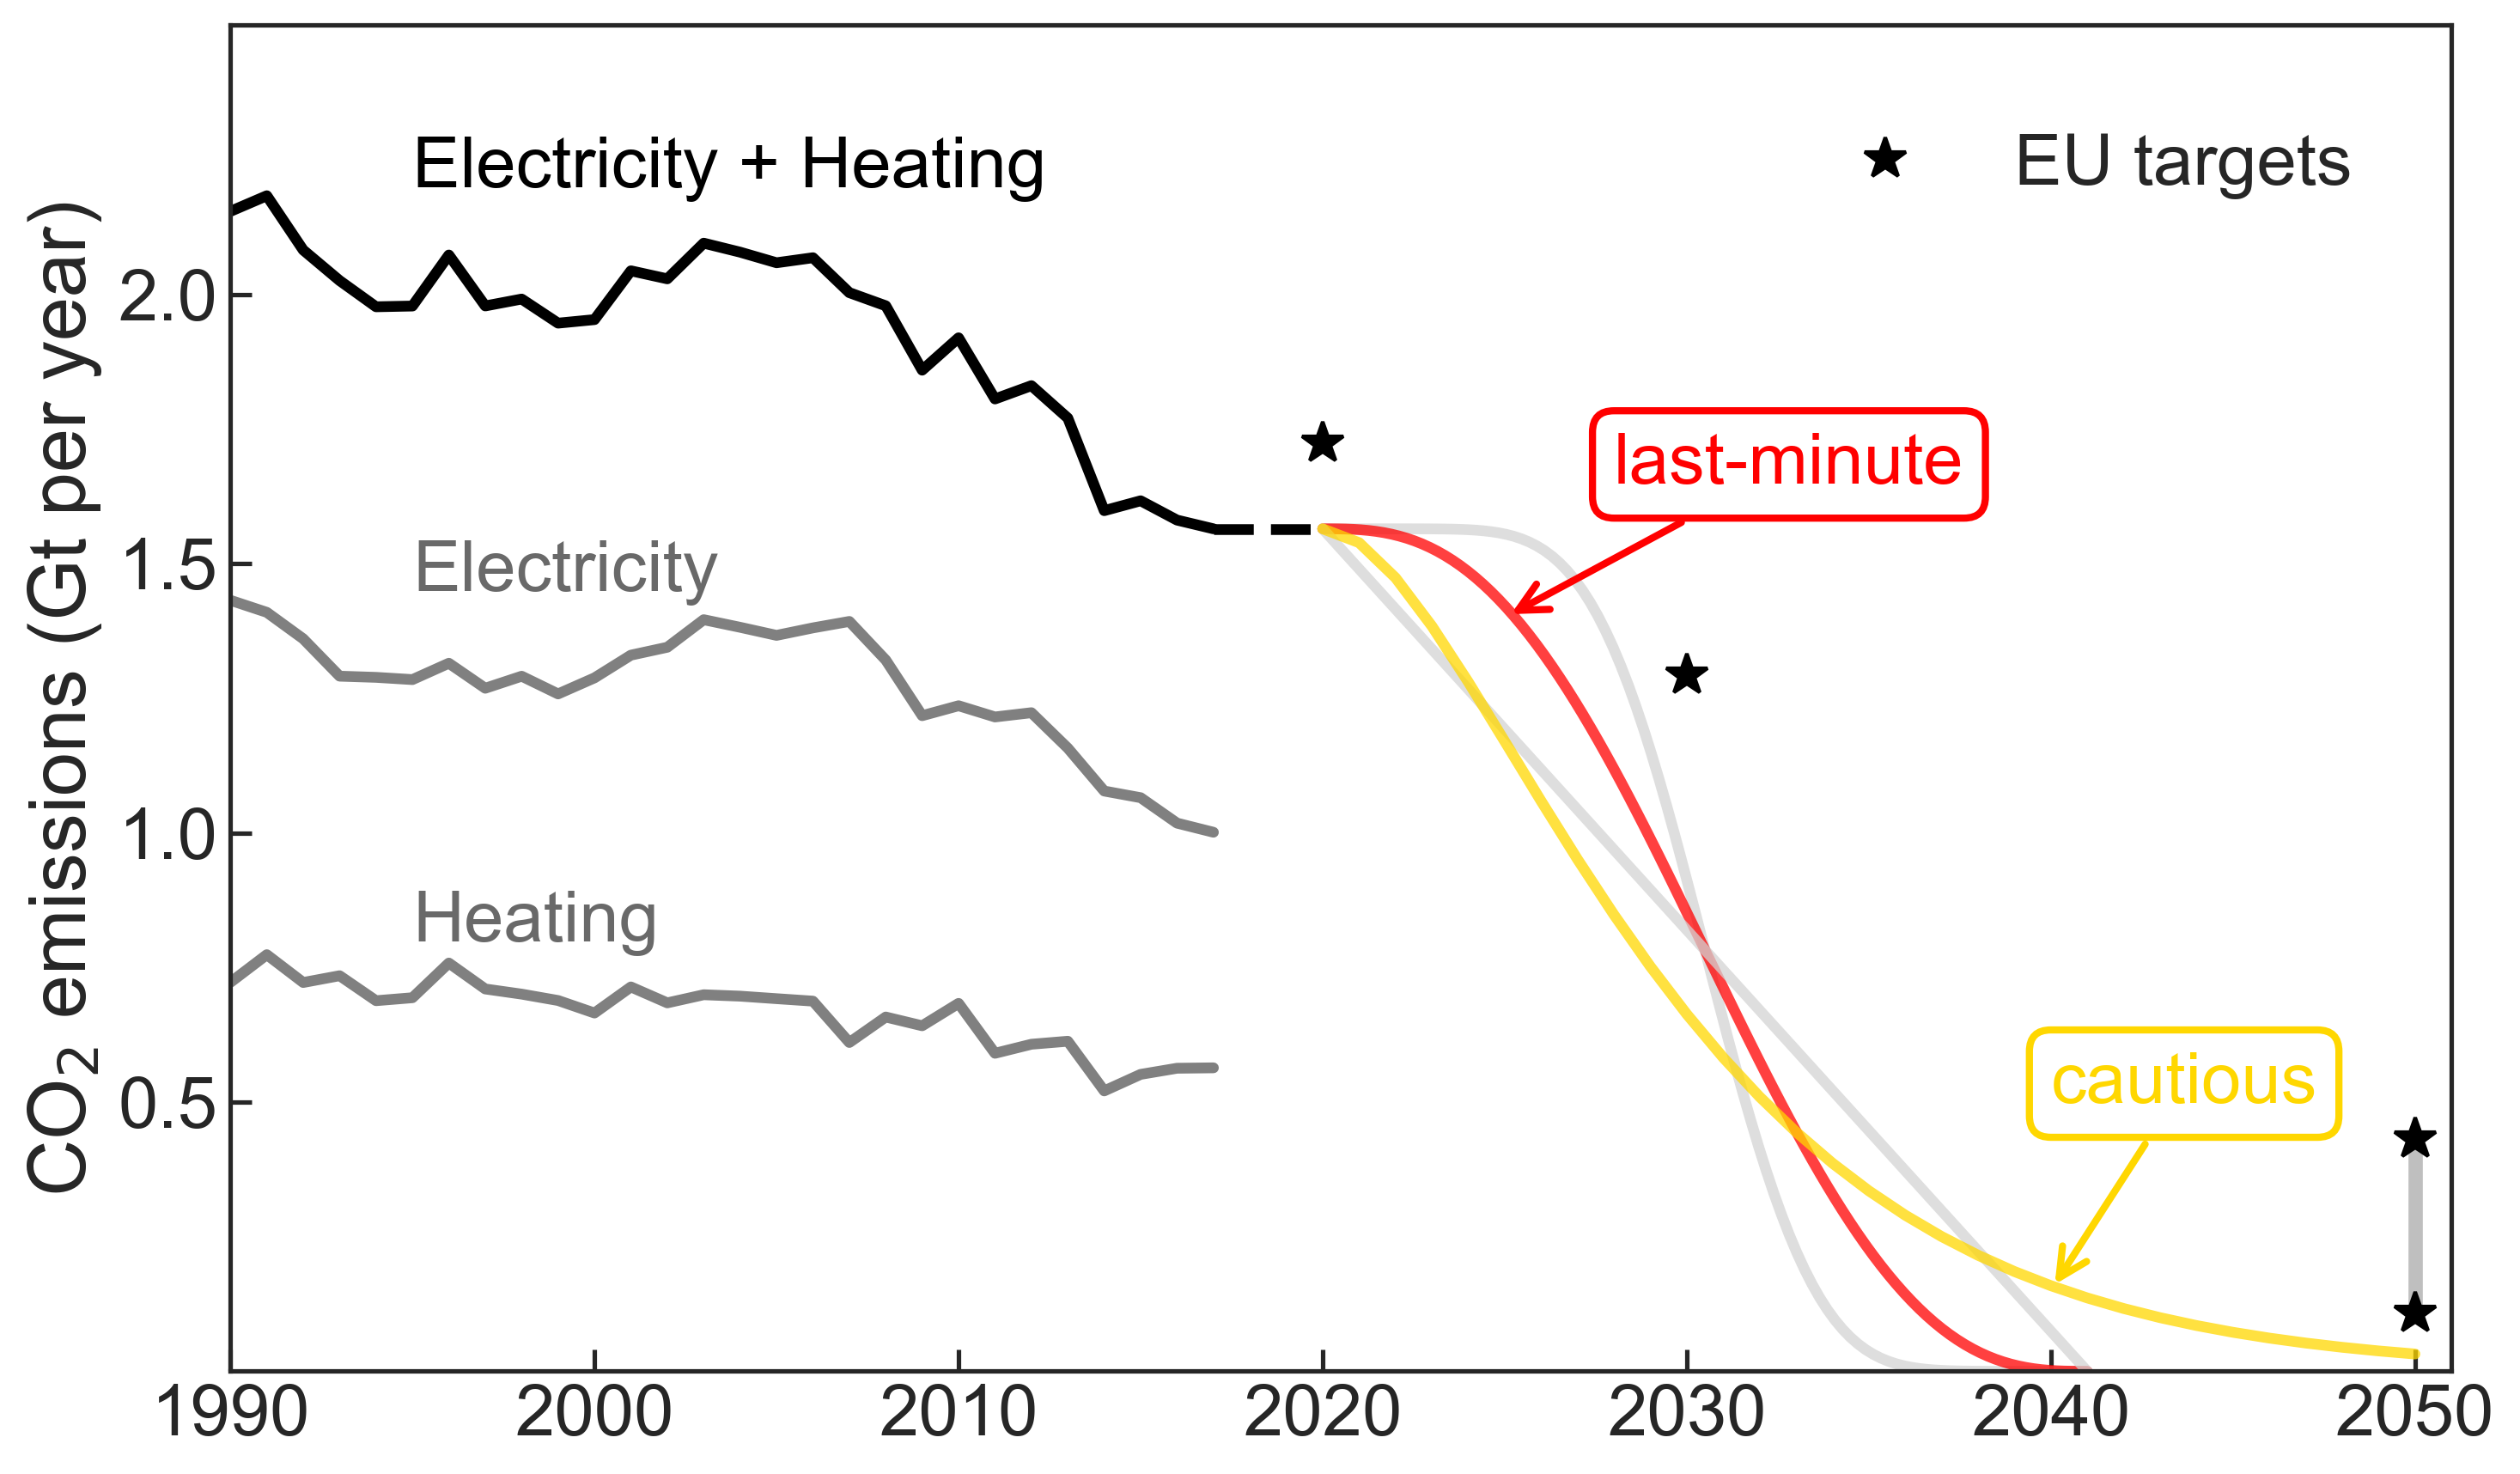
\includegraphics[width=\columnwidth]{figures/carbon_budget.png}
\caption{Historical CO$_2$ emissions from the European power system and heating supply in the residential and services sectors \cite{UNFCCC_inventory}. The various future transition paths shown in the figure have the same cumulative CO$_2$ emissions, which correspond to the remaining 21 Gt CO$_2$ budget to avoid human-induced warming above 1.75$^{\circ}$C with a probability of greater than 66\%, assuming current sectoral distribution for Europe, and equity sharing principle among regions. Black stars indicate committed EU reduction targets, while white stars mark under-discussion targets.} \label{fig_carbon_budget} 
\end{figure}

%In this work, we investigate alternative transition paths with the same cumulative CO$_2$ emissions and discuss the best way of using the remaining budget.\
In this work, we use a sector-coupled networked model of the European energy system and myopic optimisation in 5-years steps from 2020 to 2050 to investigate the impact of different CO$_2$ restriction paths with the same carbon budget. In every time step, the expansion of generation, storage and interconnection capacities in every country is allowed if it results cost-effective under the corresponding global emissions constraint. We show that realistic costs for wind and solar plus hourly resolution for balancing make climate action with renewables more cost-effective than previously seen. Furthermore, we found that a transition path with more ambitious short-term CO$_2$ targets reduces the cumulative system cost and requires more stable CO$_2$ price and build rates. Our research includes the coupling  with heating and transport sectors, contrary to existing transition paths analyses for the European power system \cite{Plesmann_2017, Gerbaulet_2019, Poncelet_2016}, as well as realistic cost assumption for wind and solar PV together with hourly resolution, contrary to most Integrated Assessment Models (IAMs) \textcolor[rgb]{1,0,0}{\cite{Creutzig_2017}}. By using an open model, we ensure transparency and reproducibility of the results in a  discipline with high policy relevance such as it is energy modelling \cite{Pfenninger_2017, Pfenninger_2018}.

\FloatBarrier

\paragraph{\textbf{Myoptic optimisation with sector coupling}} \

Electricity generation is expected to spearhead the transition spurred by the dramatic cost reduction of wind \cite{Lantz_2012} and solar photovoltaics (PV) \cite{Creutzig_2017, Haegel_2019}. A vast body of literature shows that a power system based on wind, solar, and hydro generation can supply hourly electricity demand in Europe as long as proper balancing is provided \cite{Eriksen_2017, Schlachtberger_2017, Gils_2017a, Brown_response}. This can be done reinforcing interconnections among neighbouring countries \cite{Rodriguez_2014} to smooth renewable fluctuations by regional aggregation or through temporal balancing using local storage \cite{Rasmussen_2012, Cebulla_2017, Victoria_2019_storage}. Moreover, coupling the power system with other sectors such as heating or transport could provide additional flexibilities facilitating the system operation and simultaneously helping to abate emissions in those sectors \cite{Connolly_2016, Brown_2018, Child_2019}. \\

CO$_2$ emissions from heating in residential and services sector show a more modest historical reduction trend than electricity generation (Fig. \ref{fig_carbon_budget}). Nordic countries have been particularly successful in reducing carbon emissions from the heating sector by using sector-coupling strategies (Supplementary Note 3). Denmark, where more than half of the households are connected to district heating systems \cite{Gross_2019}, has shifted the fuel used in Central Heat and Power (CHP) units from coal to biomass and urban waste incineration \cite{DEA_2015}. The high penetration of heat pumps in Sweden can be explained by a path-dependence process \cite{Gross_2019} and it is now supported by high CO$_2$ prices \cite{Carbon_pricing_2019} and low electricity taxes.\\ 

Greenfield optimisation of the future European energy system, that is, building the system from scratch, shows that sector-coupling decreases the system cost and reduces the need for extending transmission lines due to the additional local flexibility brought by heating and transport sectors \cite{Brown_2018}. Sector-coupling allows further CO$_2$ reductions before large capacities of storage become necessary, providing more time to develop further storage technologies \cite{Victoria_2019_storage}. Greenfield optimisation is useful to investigate the optimal configuration of the fully-decarbonised system, but it does not provide insights on how to transition towards it. Today's generation fleet and decisions taken in intermediate steps will shape the final configuration. Transition paths for the European power system have been analysed using myopic optimisation, without full foresight over the investment horizon \cite{Bogdanov_2019, Plesmann_2017, Gerbaulet_2019, Poncelet_2016}. Myopic optimisation results in higher cumulative system cost than optimising the entire transition period with perfect foresight because the former leads to stranded investments \cite{Gerbaulet_2019, Heuberger_2018}. However, the myopic approach is less sensitive to the assumed discount rate and can capture better short-sighted behaviour of political actors and investors. 

%\paragraph{\textbf{Carbon budget for electricity and heating in Europe}} \
\paragraph{\textbf{Alternative transition paths}} \
\subparagraph{\textbf{Cumulative costs}} \

Here, we investigate the consequences of following two alternative transition paths. The Gentle path represents a cautious approach in which significant emissions reductions are attained in the early years. In the Sudden path, the low initial reduction targets quickly deplete the carbon budget requiring a sharp reduction later. As in Aesop's fable, making fun of the cautious tortoise, following the hare strategy and delaying climate action requires a later speeding up that will be more expensive and might be unfeasible.  \

The two alternative paths arrive at a similar system configuration in 2050. Towards the end of the period, under heavy CO$_2$ restriction, balancing technologies appear in the system. They include large storage capacities comprising electric batteries and hydrogen storage, and methanation.  \textcolor[rgb]{1,0,0}{Cumulative cost for the Gentle path represents 7,869 billion euros (B\EUR), while the Sudden path accounts for 8,211 B\EUR.} The newly built conventional capacity for electricity generation is very modest in both cases, Fig. \ref{fig_age_distribution} and Supplementary Note 9. Decarbonising the power system has proven to be cheaper than the heating sector \cite{Zhu_2019}. Consequently, although CO$_2$ allowances differ, the electricity sector gets quickly decarbonised in both paths. \textcolor[rgb]{1,0,0}{More notable differences appear in new conventional heating capacities, Fig. \ref{fig_heating_expansion}. Regarding new renewable generation and power-to-heat capacities, both paths show major differences.}

\subparagraph{\textbf{Stranded assets}} \

\textcolor[rgb]{1,0,0}{Although conventional electricity generators do not extend significantly, the already existing capacities become stranded assets. Utilisation factors for gas power plants drop, Supplementary Note 8, and market revenues are not enough to recover costs at any point, Fig \ref{fig_revenue_vs_expenditure}. This is a consequence of the large capacity of gas recently installed in Europe. Fig. \ref{fig_age_distribution} shows that most of the gas capacity in Europe was installed less than 25 years ago, part of this capacity represents a stranded asset for both transition paths. Although, infrautilisation of existing generation capacity might be seen as an unnecessary contribution to a higher cost of energy it must be remarked that the early retirement of electricity infrastructure has been identified as one of the most cost-effective actions to reduce committed emissions and enable a 2$^{\circ}$C-compatible future evolution of global emissions \cite{Tong_2019}.}

%This is a consequence of the role that gas units play as backup technology securing electricity and heat supply when there is a significant deficit of renewable generation, but it is also a consequence of the large capacity of gas recently installed in Europe. OCGT and CCGT gas power plants represent the main stranded assets causing the higher cost in the later. The higher CO$_2$ emissions allowance in 2030 and earlier allow the installation of such plants. However, the drastic change in emissions restriction in subsequent years, avoids the operation of gas power plants. The Europe-averaged utilisation factors shown in Fig. \ref{fig_utilisation_factors} are close to zero from 2040 onwards for the gas units in the Hare path, and they recover less than X\% of their cost via market revenues. For both transition paths, even in the initial years the utilisation factor of gas is below 50\%. 

\begin{figure*}[!h]
\centering
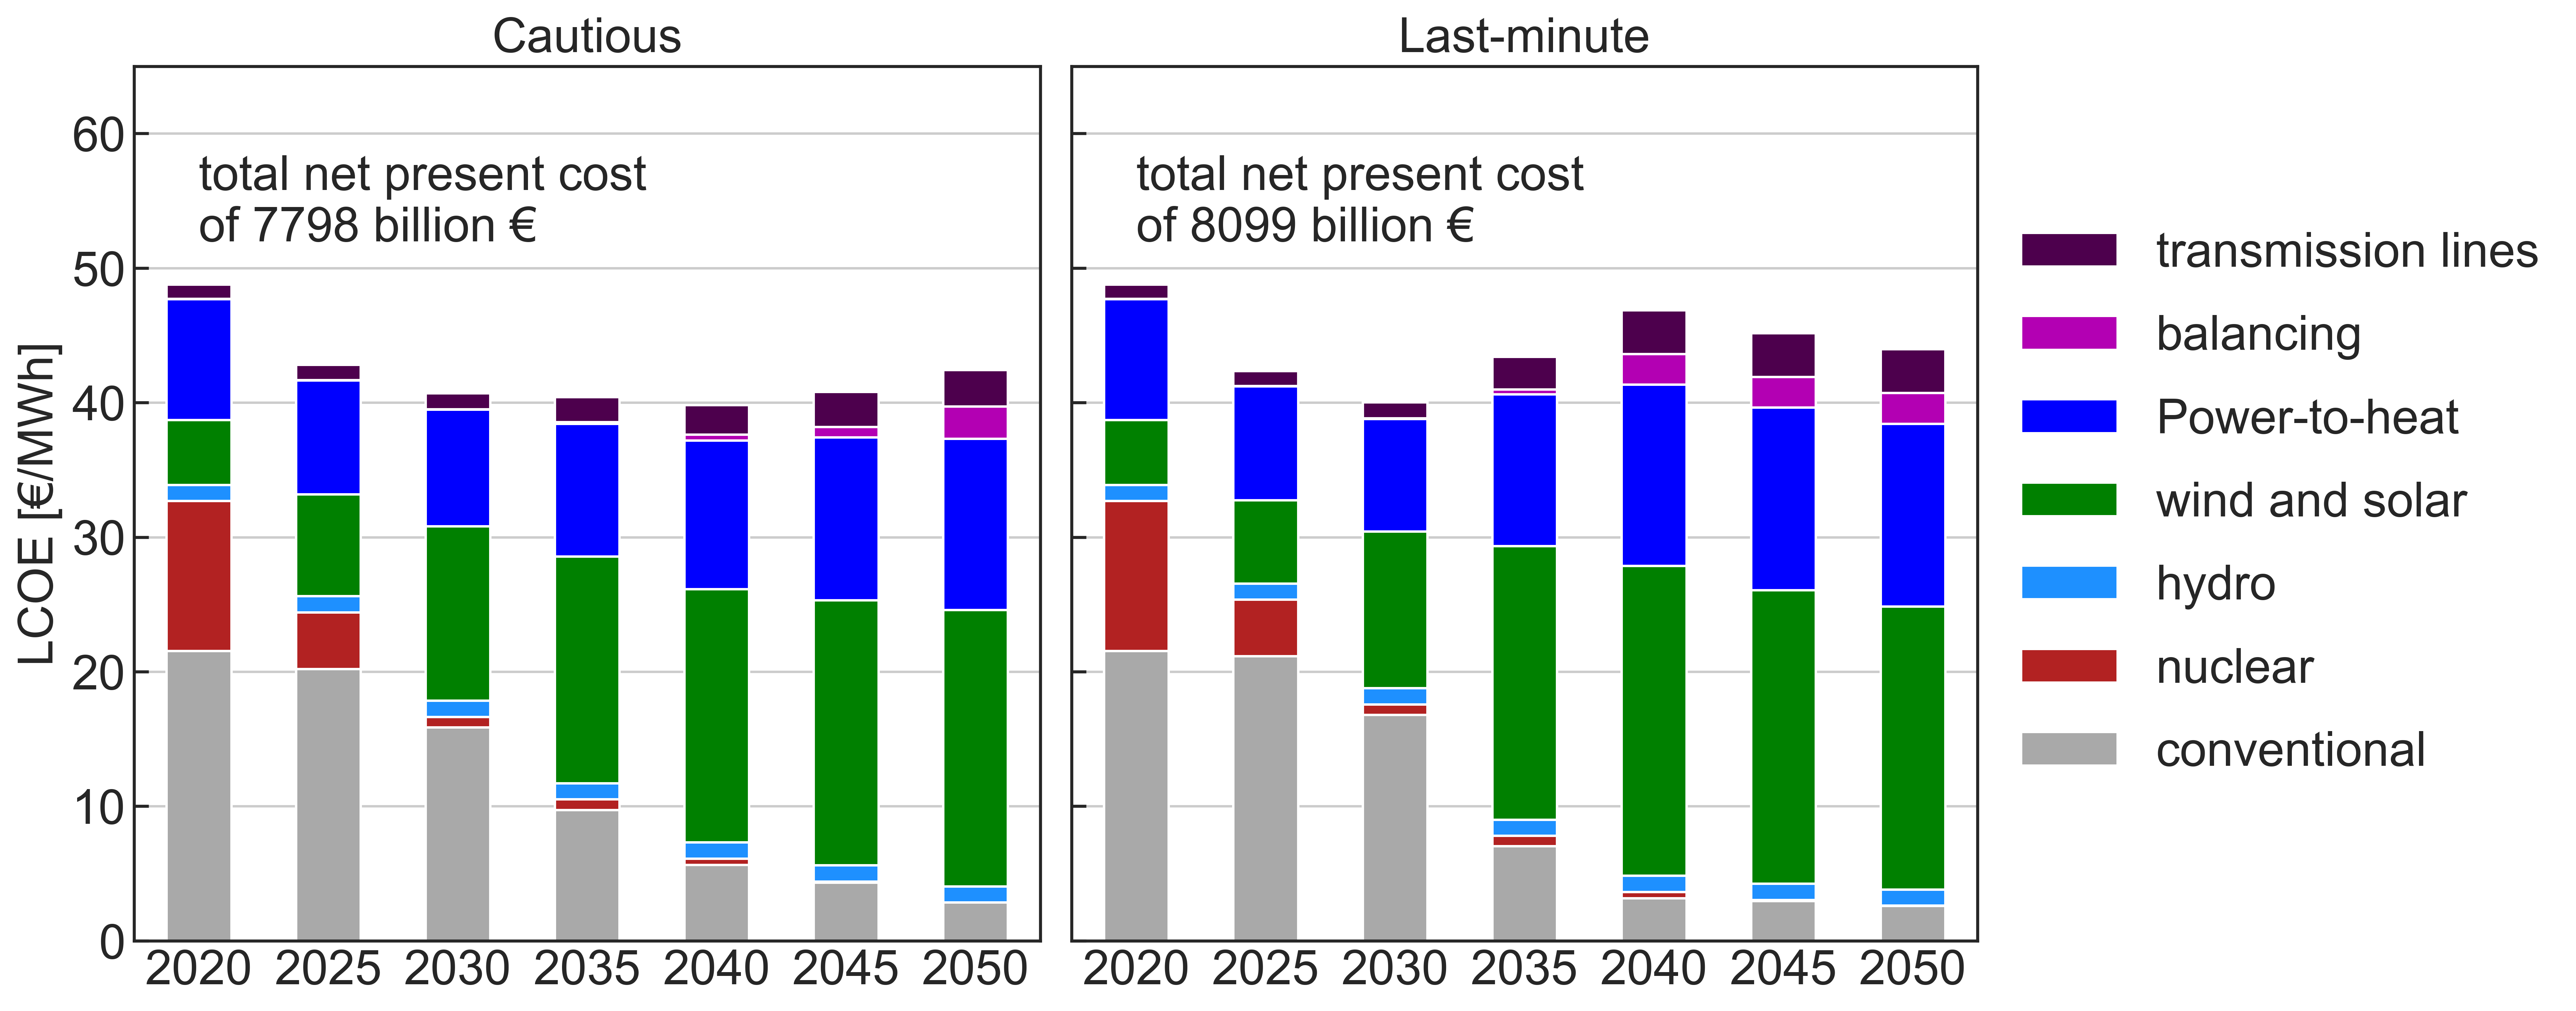
\includegraphics[width=14cm]{figures/LCOE_Base.png}
\caption{\textcolor[rgb]{1,0,0}{Levelized Cost of Energy (LCOE) for the European electricity and heating system throughout transition paths Gentle and Sudden shown in Fig. \ref{fig_carbon_budget}. Conventional includes costs associated with coal, lignite, and gas power plants producing electricity as well as costs for fossil-fueled boilers and CHP units. Power-to-heat category includes costs associated with heat pumps and heat resistors. Balancing includes cost of electric batteries, H$_2$ storage, and methanation. }} \label{fig_system_cost} 
\end{figure*}

\begin{figure*}[!h]
\centering
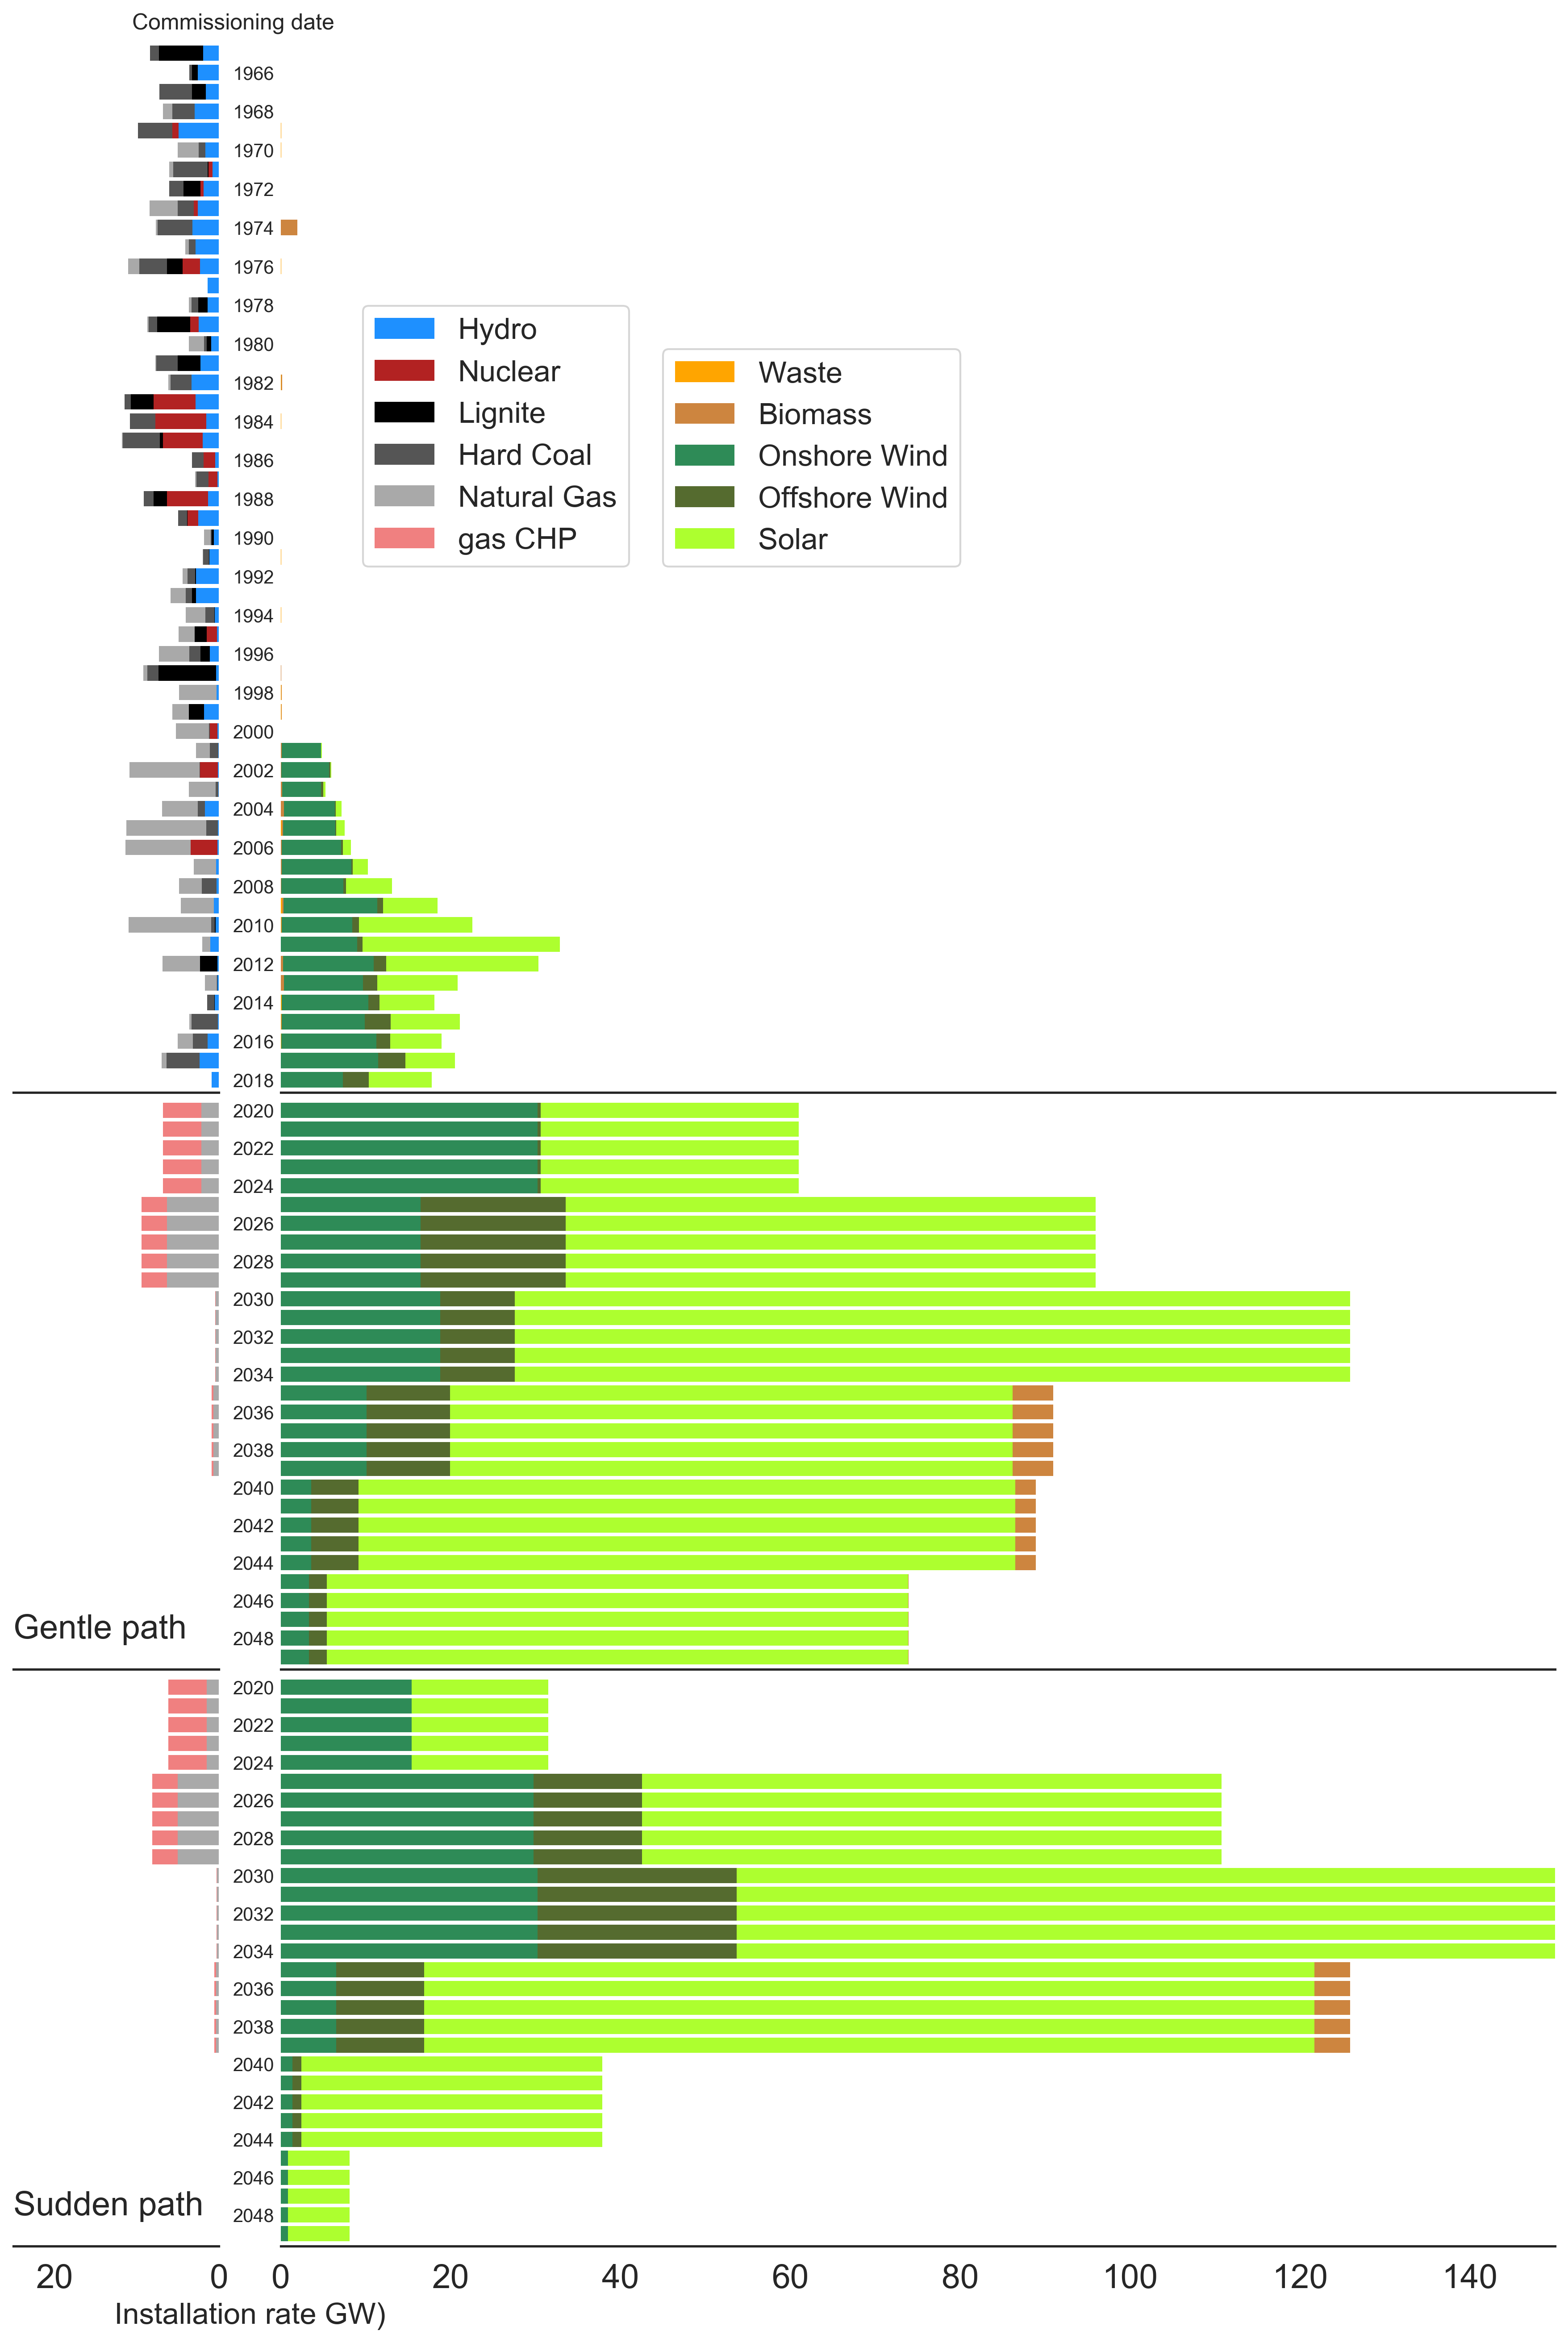
\includegraphics[width=0.8\textwidth]{figures/age_distribution_Base.png}
\caption{Age distribution of European power plants in operation \cite{powerplantmatching, IRENA_2019} and required annual installation throughout the Gentle path.} \label{fig_age_distribution} 
\end{figure*}

\begin{figure*}[!h]
\centering
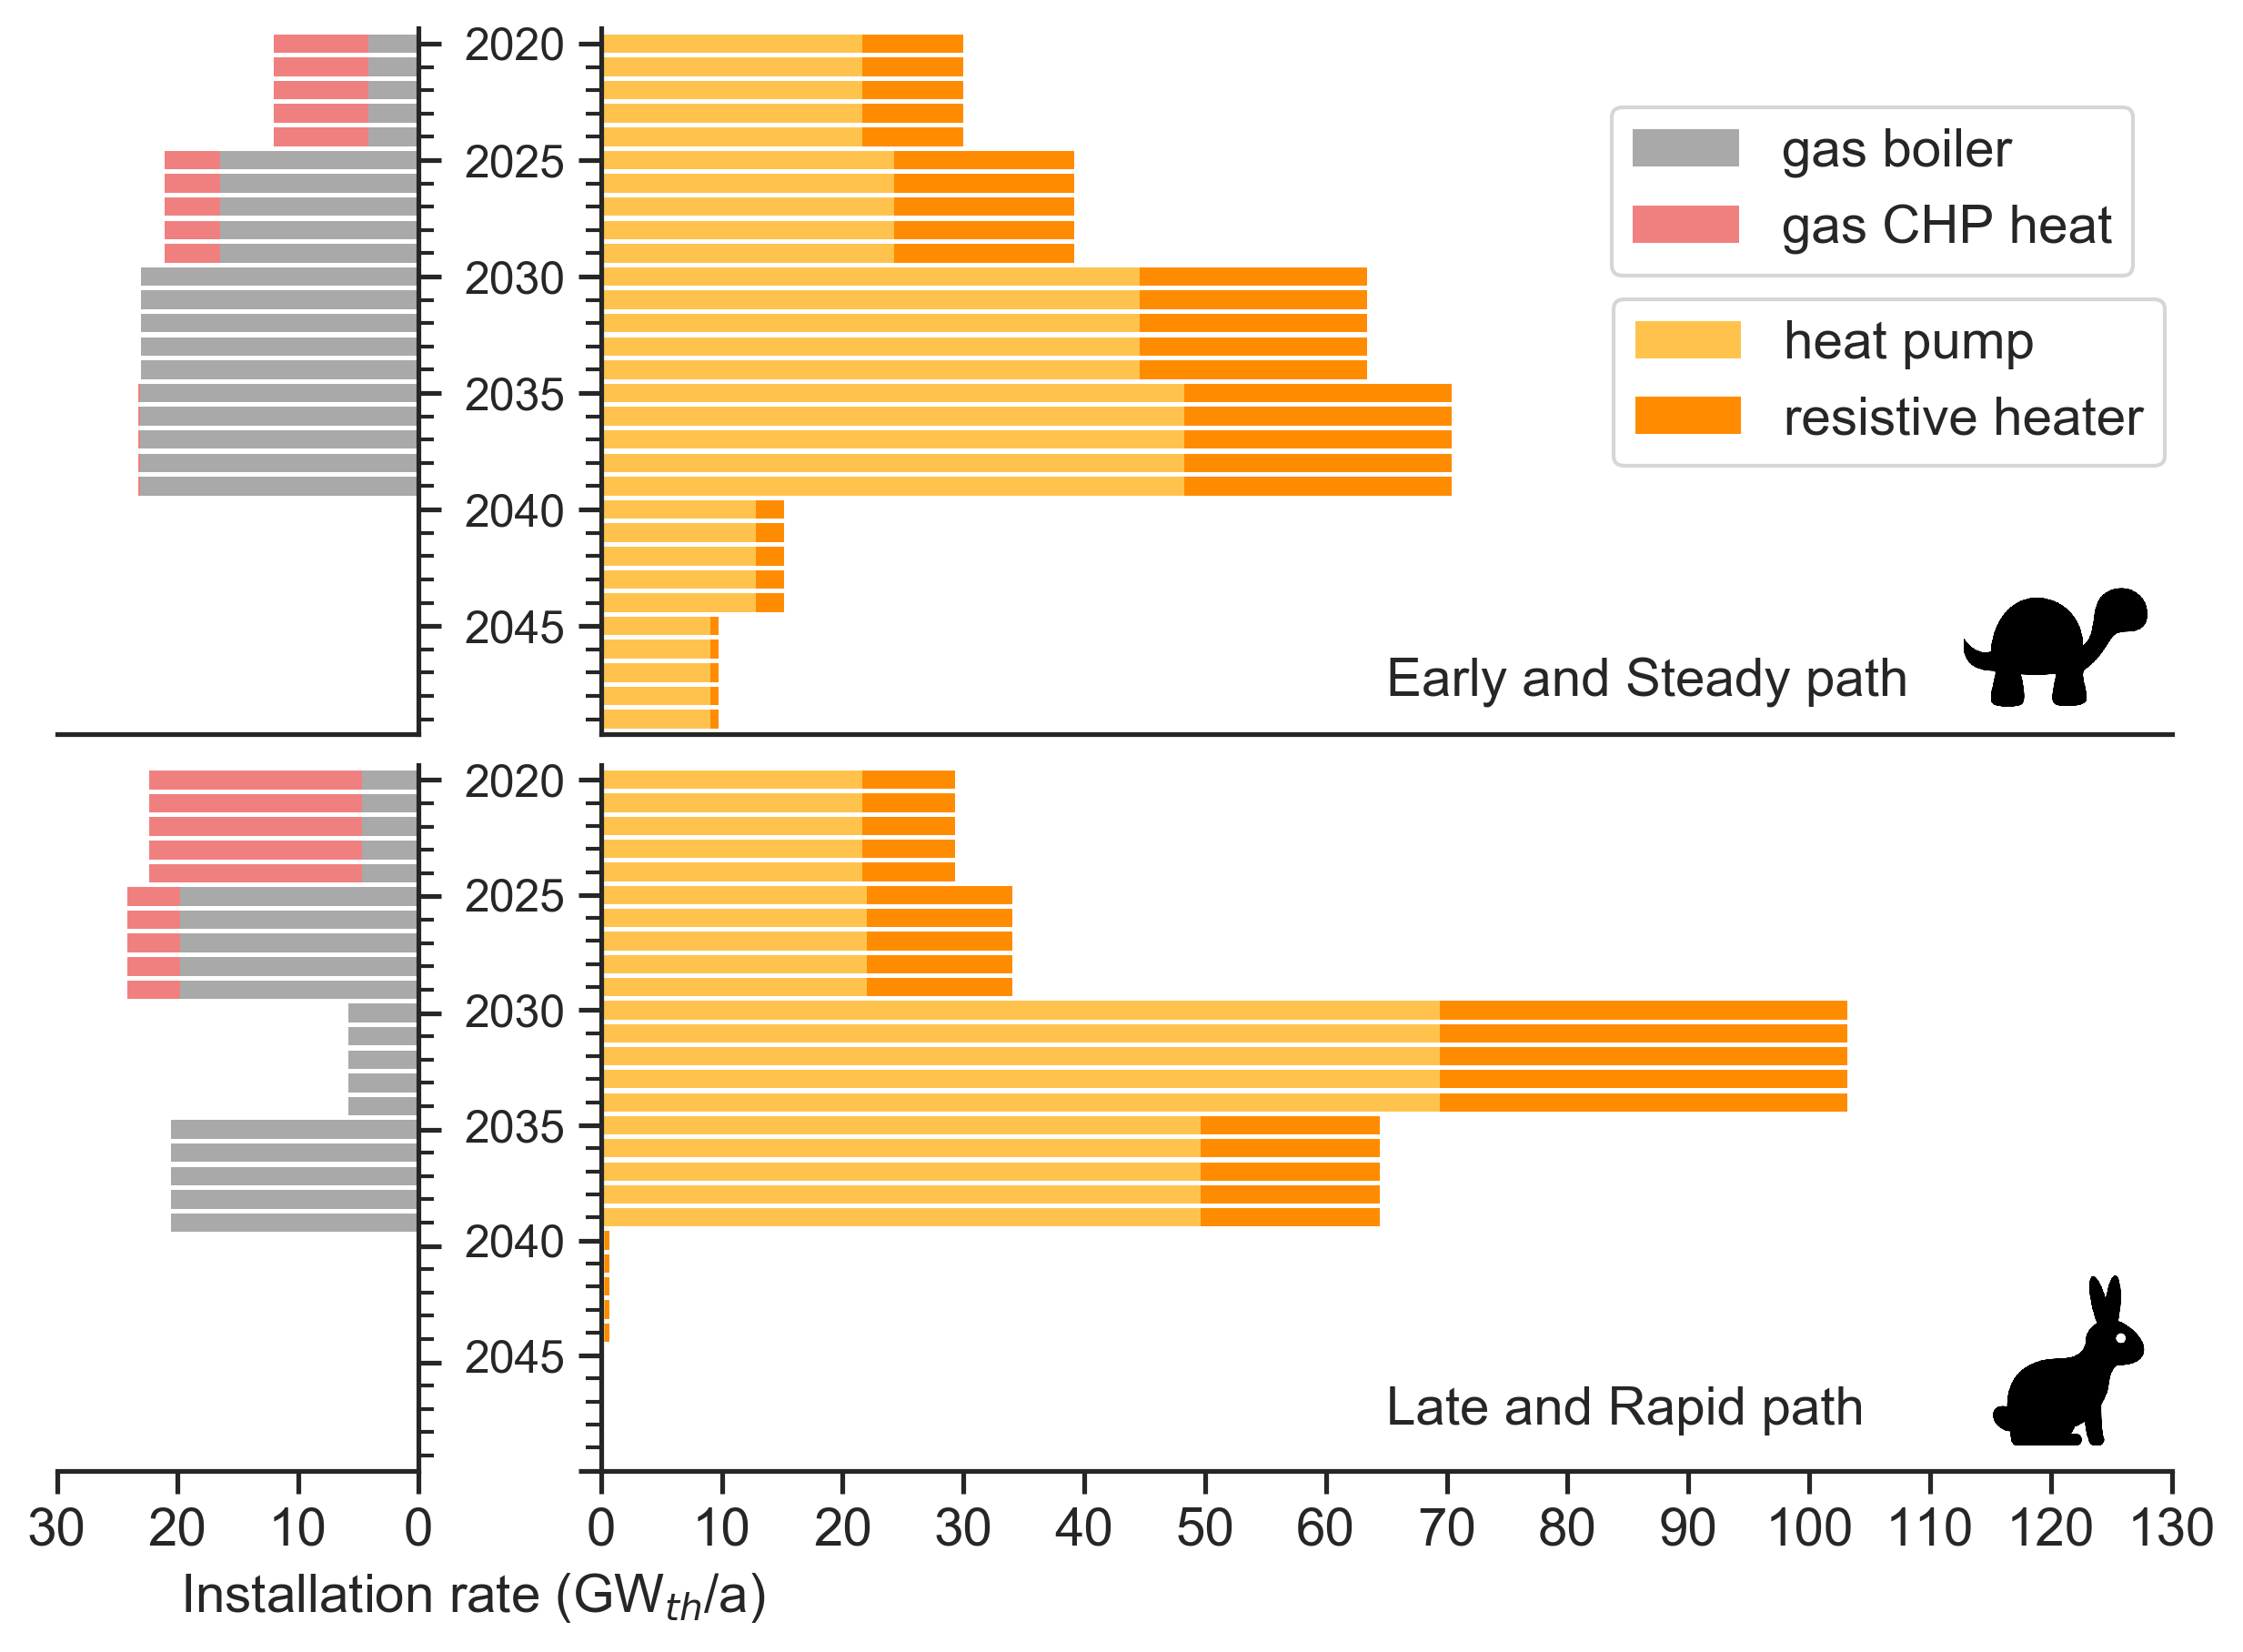
\includegraphics[width=0.8\textwidth]{figures/heating_expansion_Base.png}
\caption{Required heating capacities expansion in both paths.} \label{fig_heating_expansion} 
\end{figure*}

\begin{figure}[!h]
\centering
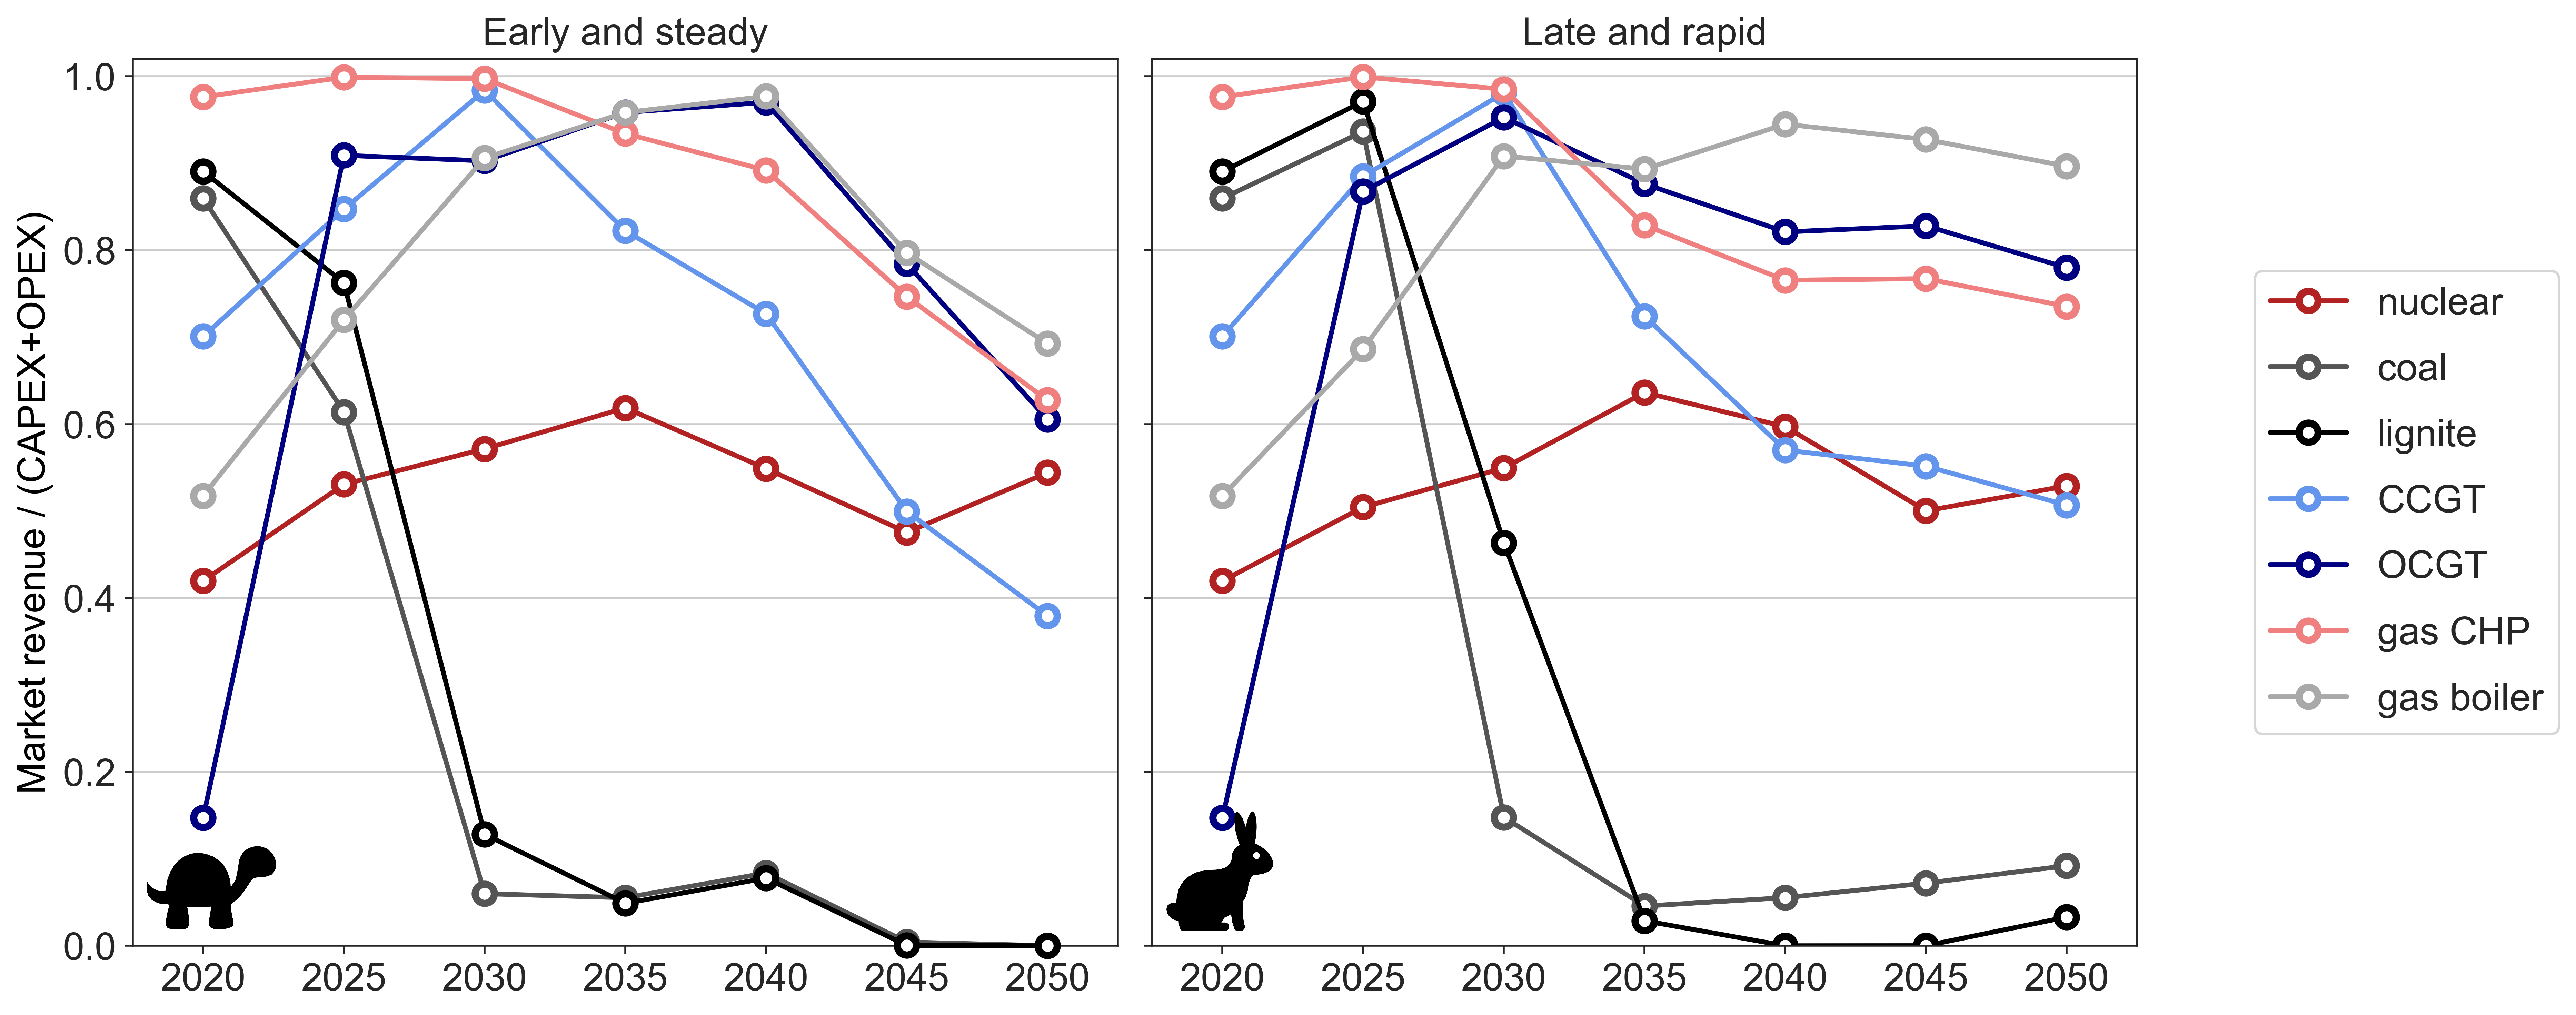
\includegraphics[width=\columnwidth]{figures/revenue_vs_expenditure_Base.png}
\caption{Ratio of market revenues to total expenditure for lignite, coal, gas, and nuclear power plants throughout transition paths shown in Fig. \ref{fig_carbon_budget}. } \label{fig_revenue_vs_expenditure} 
\end{figure}

%\paragraph{\textbf{Build rates and feasibility of transition paths}} \
%\paragraph{\textbf{Policy incentives are needed}} \
\subparagraph{\textbf{Transition smoothness}} \

A timely transition is challenging yet doable. Decarbonising the electricity and heating sector using wind and solar PV requires duplicating the historical \textcolor[rgb]{1,0,0}{maximal} build rates, Fig. \ref{fig_age_distribution} and Supplementary Note 4. Consequently, attaining higher build rates to also decarbonise transport and industry sectors seems possible.\textcolor[rgb]{1,0,0}{ Wind and solar PV provides 45\% and 40\% respectively of the electricity demand in 2050}, complemented by hydro generation. Previously, most IAMs have emphasized the importance of bioenergy or carbon capture and storage and failed to identify the key role of solar PV due to their unrealistically high cost assumptions for this technology, see \cite{Creutzig_2017, Krey_2019} and Supplementary Note 8. \\

During the past decade, several European countries have shown sudden increments in the annual build rate for solar PV, followed by equivalent decrements one or two years later. Italy, Germany, Spain, and UK show clear peaks (see Supplementary Note 4)  due to the combination of a fast cost decrease of the technology and unstable regulatory frameworks whose details are country-specific. These peaks are lethal for local businesses. The sudden shrinkage of annual build capacity results into companies bankruptcy and job loss. The Gentle transition path requires a smoother evolution of build rates which could better accommodate the cultural, political, and social aspects of the transition \cite{Geels_2017}. \\ %Although none of the build rates required in the Sudden path is technological infeasible, the Gentle path is more compatible with the inertias in the transition such as required time to modify regulatory frameworks or to educate the necessary labour force. 

CO$_2$ prices much higher than those historically attained in the ETS market are necessary throughout the transition, Fig. \ref{fig_co2price}. The Gentle path requires smoother evolution of CO$_2$ price which will have a positive impact on investors. Due to its large seasonal variation, decarbonisation of the heating sector is known to require higher CO$_2$ prices than the electricity sector, mainly to push into the system high-efficiency but capital-expensive technologies such as heat pumps \cite{Brown_2018, Victoria_2019_storage}. CO$_2$ price is only an indication of the price gap between polluting and clean technologies and several policies can be established to fill that gap. Among others, sector-specific CO$_2$ taxes \cite{Carbon_pricing_2019}, auctions for renewable capacity that reduce the risk, and consequently the WACC and LCOE of the technology \cite{Vartiainen_2019}, or regulatory frameworks that incentivise the required technologies such those promoting rooftop PV installations or ensuring the competitiveness of district heating systems. %Several remarks are worth it. First, CO$_2$ price is impacted by the model assumptions and lower values could be obtained if, for example, a lower cost were assumed for biomass. 


\begin{figure}[!h]
\centering
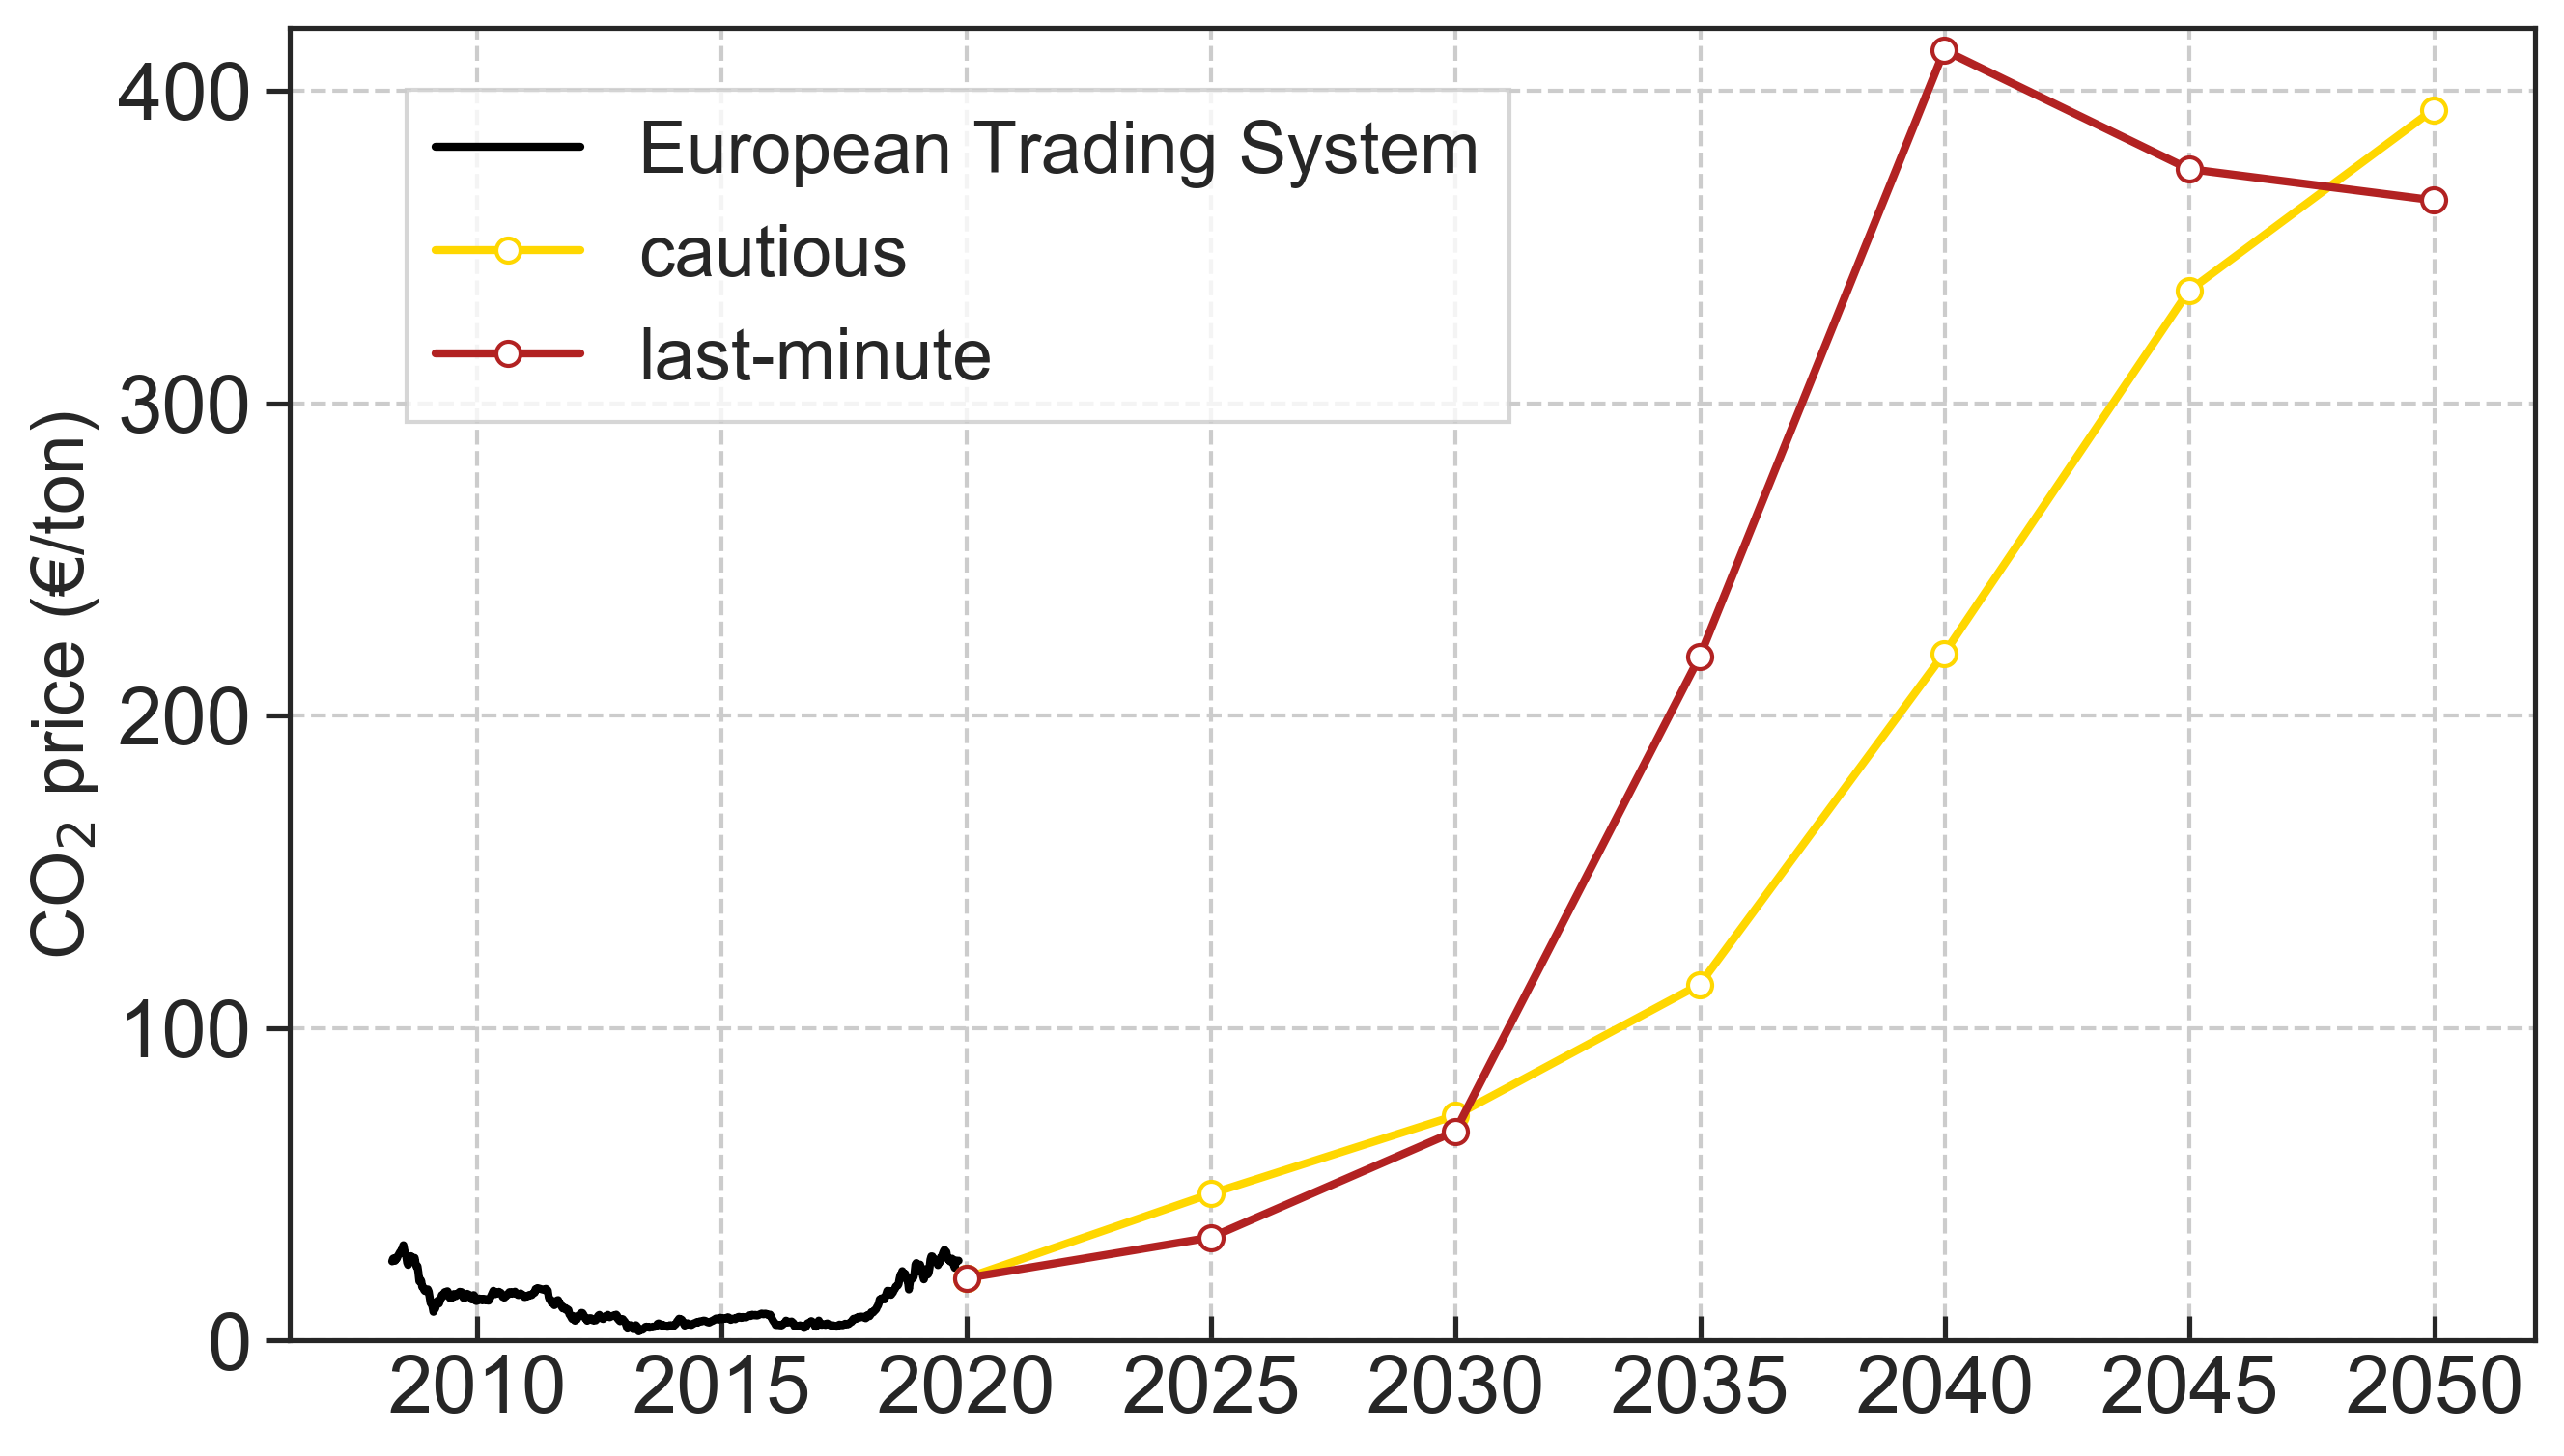
\includegraphics[width=\columnwidth]{figures/co2_price.png}
\caption{Historical evolution of CO$_2$ price in the European Trading System \cite{ETS} and required CO$_2$ price obtained from the model throughout transition paths shown in Fig. \ref{fig_carbon_budget}} \label{fig_co2price} 
\end{figure}
\FloatBarrier

\paragraph{\textbf{Hourly time resolution and renewable balancing}} \

Modelling an entire year with hourly resolution unveils the strong links among renewable generation technologies and balancing strategies. For countries and time steps in which large solar PV capacities are deployed, it is also cost-effective to install large battery capacities to smooth the strong daily solar generation pattern. Conversely, onshore and offshore wind capacities require H$_2$ storage and reinforced interconnections to balance wind synoptic fluctuations \cite{Rasmussen_2012, Rodriguez_2014, Schlachtberger_2017, Victoria_2019_storage}. %The strong bounds existing between solar PV-battery and wind-hydrogen  
This can also be appreciated by looking at the dominant dispatch frequencies exposed by the Fourier power spectra of the dispatch time series, Fig. \ref{fig_Fourier}. \
IAMs with similar spatial resolution than our model, \textit{i.e.}, one node per country, have also been used to investigate the sector-coupled decarbonisation of Europe \cite{in-depth_2018, JRC-EU-TIMES, Creutzig_2017}. However, IAMs typically use a much lower time resolution, \textit{e.g.}, using a few time slices to represent a full year \cite{JRC-EU-TIMES, Loffler_2019, Poncelet_2016, McGlade_2015, Babrowski_2014} or considering the residual load duration curve \cite{Creutzig_2017, Ueckerdt_2017}. The hourly resolution in our model unveils several effects that are critical to the operation of highly renewable systems, such as the solar and wind non-correlations smoothed by the grid, the role of long-term storage, and the system operation during cold spells, \textsl{i.e.}, a cold week with low wind and solar generation.

\begin{figure}[!h]
\centering
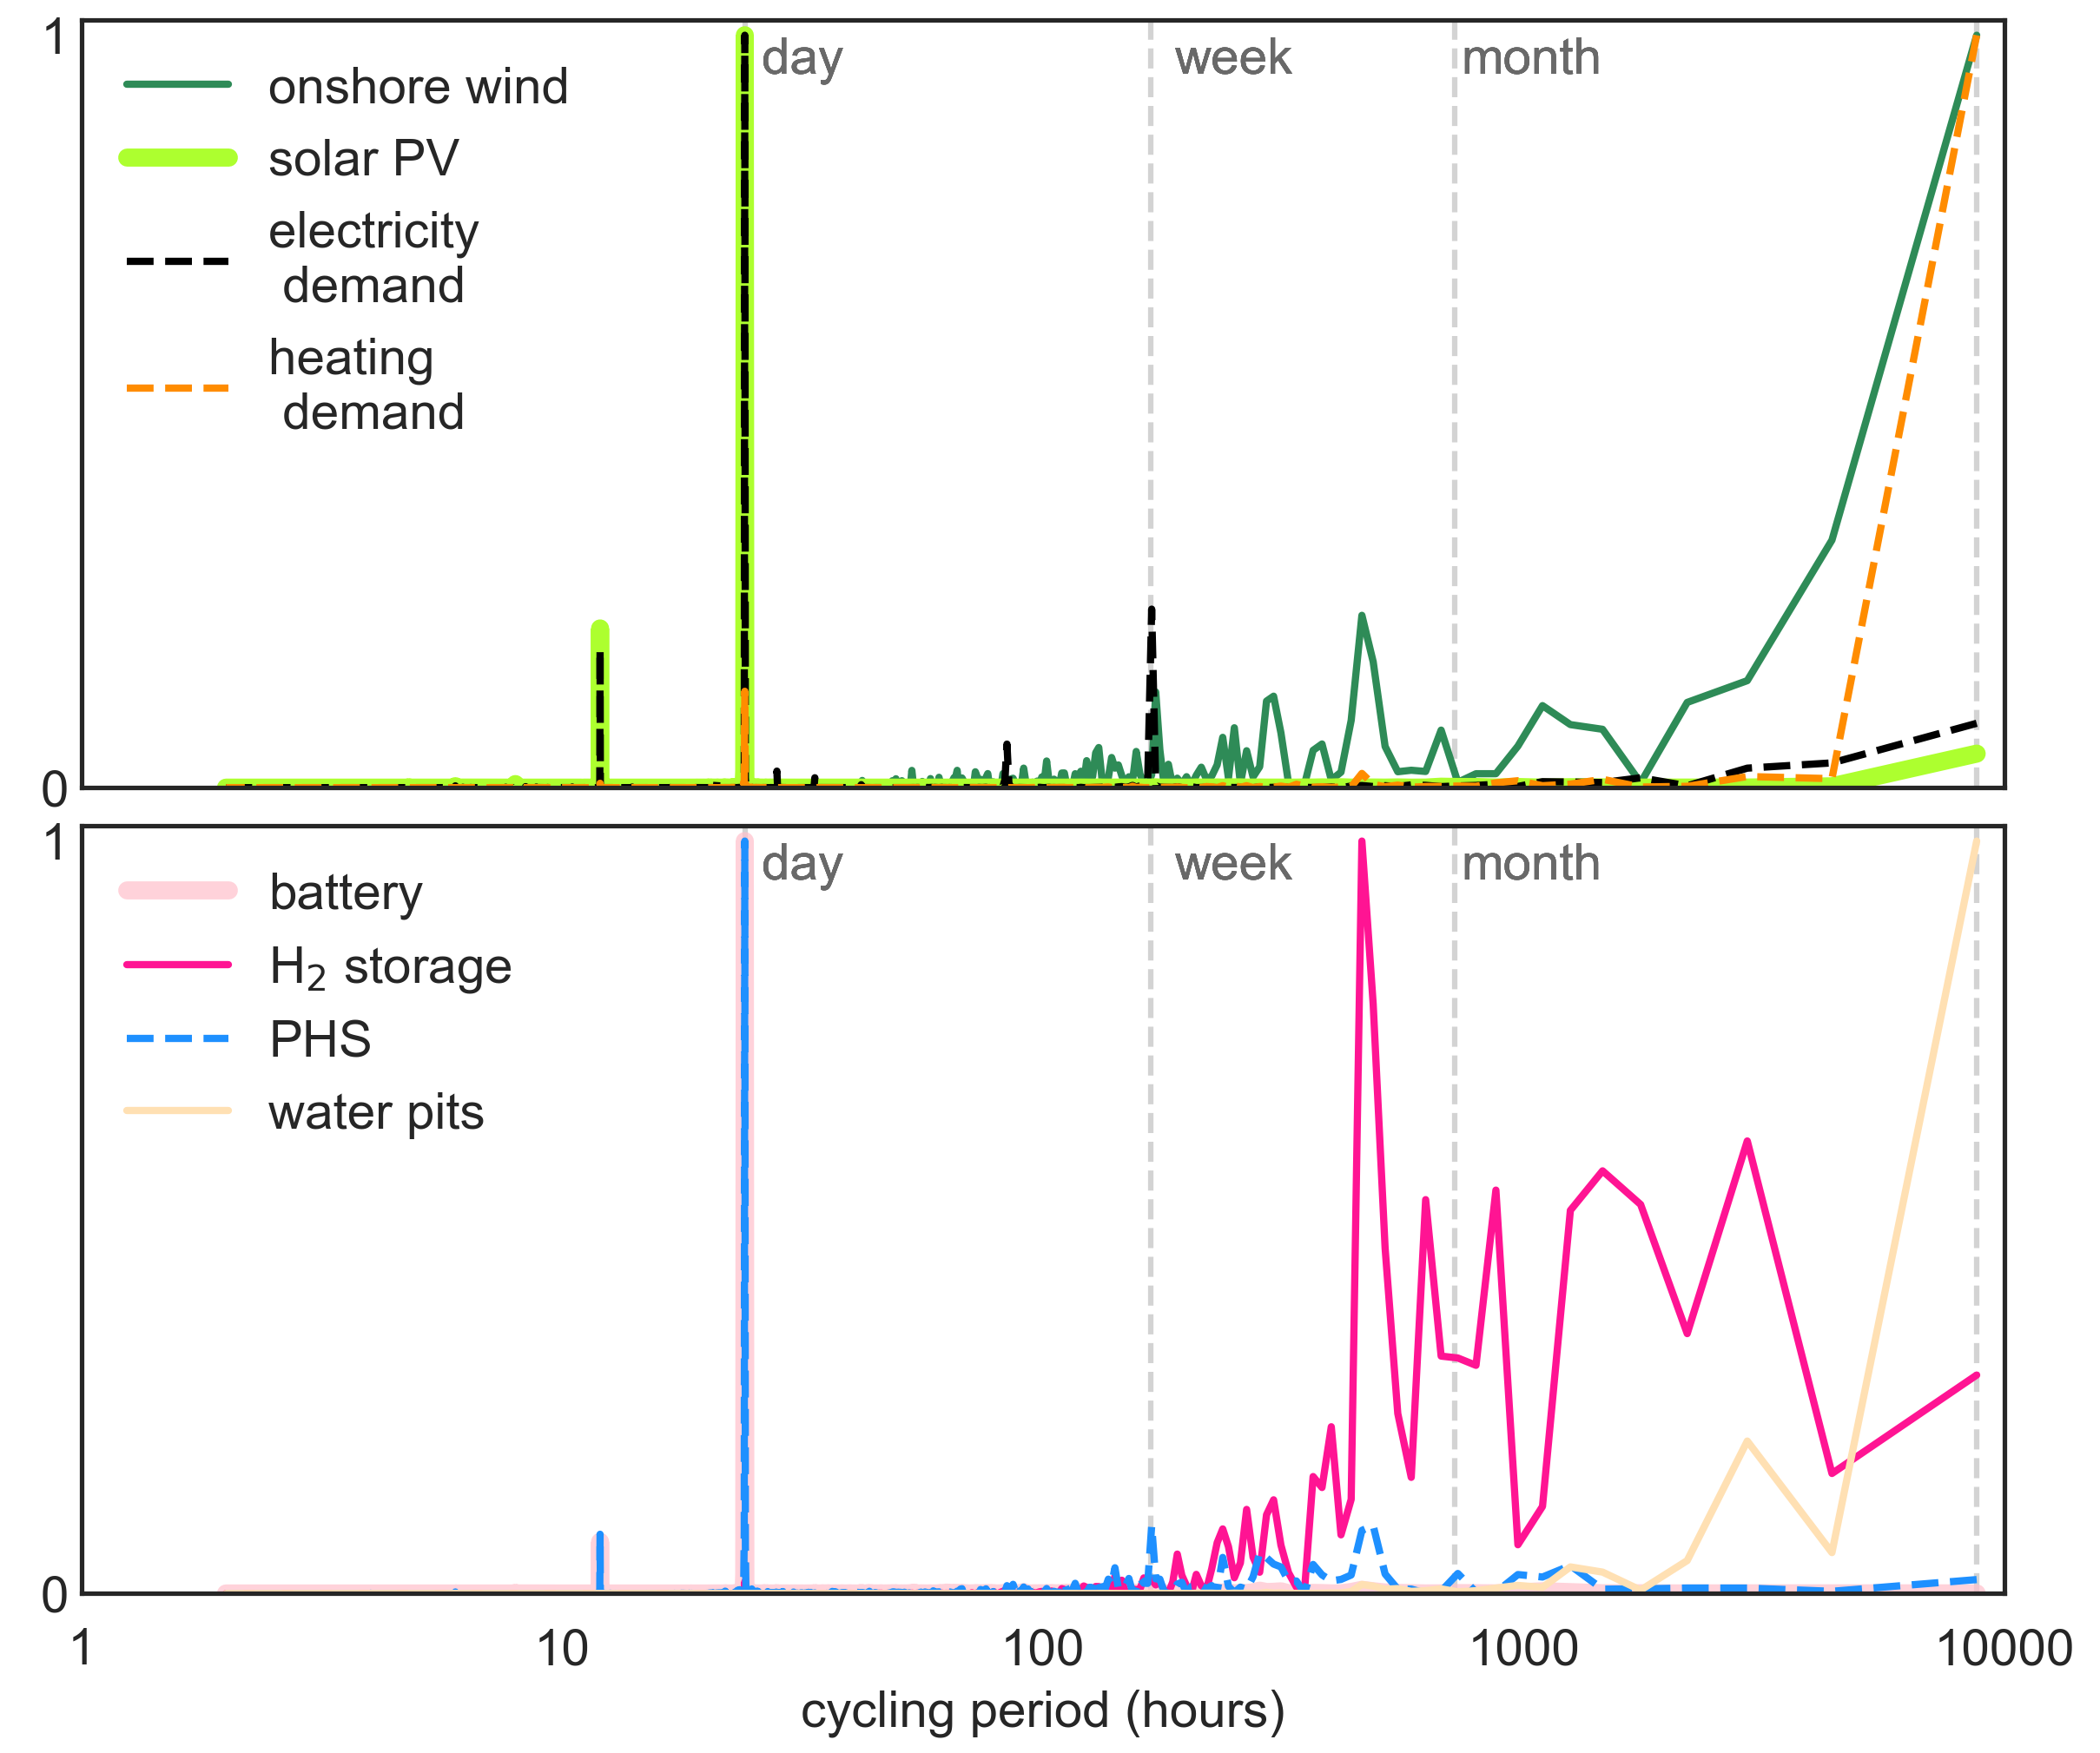
\includegraphics[width=\columnwidth]{figures/Fourier.png}
\caption{Fourier power spectra of wind and solar PV generation, electricity and heating demand, as well as storage technologies dispatch time series. The time series represent the Europe-aggregated generation/demand for \textcolor[rgb]{1,0,0}{the Gentle path in 2050. (poner heating demand en naranja)}} \label{fig_Fourier} 
\end{figure}


The optimal renewable mix in every country depends on the local resources and the already existing capacities, see Fig. 14 in Supplementary Note 9. Nevertheless, it should be remarked that the analysis of near-optimal solutions has recently shown that country-specific mixes can vary significantly while keeping the total system cost only slightly higher than the minimum \cite{Neumann_2019}. 

\FloatBarrier
 
\paragraph{\textbf{ Transport?}} \

District heating (DH) has proven to be extremely useful to decarbonise the heating sector. It allows cheaper centralised technologies such as heat pumps and CHP units, enables a faster conversion because it is easier to substitute one central heating unit than a myriad of individual domestic systems, and facilitates long-term thermal energy storage, via cheap large water pits, Fig.\ref{fig_Fourier}, that help to balance the large seasonal variation of heating demand, Supplementary Note 6. When DH is assumed to expand linearly so that it supplies the entire urban heat demand in every country, cumulative system cost for the Gentle path reduces by 259 B\EUR which roughly offsets the cost of extending and maintaining the DH networks and avoids the additional expansion of gas distribution networks. When a 2\% reduction of space heating per year is assumed due to the retrofitting of building stock, cumulative system cost decreases by 858 B\EUR compared to paths with constant heating demand. When the model is allowed to optimised transmission capacities after 2030 together with the generation and storage assets, the optimal configuration at the end of the paths includes transmission volume approximately three times larger than that of 2030. Although the cumulative system cost is 79 B\EUR lower, it is unclear that it compensates the social acceptance issues associated with increasing transmission capacities. 

\paragraph{\textbf{Conclusions}} \

When comparing alternative transition paths for the European energy system with the same carbon budget, we found that those including a gentle CO$_2$ reduction path are considered around 300 B\EUR cheaper than those paths where low targets in the initial period demand a sharper reduction later. These findings could contribute to the on-going discussing regarding increasing CO$_2$ reduction targets for 2030. Early action not only allows room for decision-making later but it is also found to pay off.  
% These findings support the need for ambitious climate action in the near term in a European.


%\paragraph{\textbf{The challenging decarbonisation of the heating sector}} \
%District heating has proven to be extremely useful to decarbonise the heating sector. It allows cheaper centralised technologies such as heat pumps and CHP units, and makes possible a fast conversion because it is easier to substitute one central heating unit than a myriad of individual domestic systems. On top of that, district heating enables long-term thermal energy storage, via cheap large water pits, Fig.\ref{fig_Fourier}, that help to balance the large seasonal variation of heating demand, Supplementary Note 6. Previously, district heating penetration in every country was kept fixed at its value in 2015 \cite{DH_penetration} throughout the entire paths. When district heating is assumed to expand linearly so that in 2050 it covers the entire urban heat demand in every country, cumulative system cost for the Gentle path reduces by 13 B\EUR. Although the additional cost of extending and maintaining the required district heating networks can be estimated in 10 B\EUR/year \cite{Brown_2018} including in the calculation the avoided expansion of gas distribution networks when district heating is deployed, makes this option certainly cheaper. 

%\paragraph{\textbf{Impact of building retrofitting}} \
%Retrofitting building stock at a rate of 2\% have been observed in the past \cite{agora}\textcolor[rgb]{1,0,0}{check reference}. Assuming a 2\% reduction of space heating per year and neglecting any rebound effect, this will translate into an aproximatlely decrease of 40\% of heating demand in 2050. Cumulative system cost decreases by \textcolor[rgb]{1,0,0}{X} \EUR compared to the paths with constant heating demand.

%\paragraph{\textbf{Transitioning without grid expansion}} \
%When the model is allowed to optimised transmission capacities after 2030 together with the generation and storage assets, the optimal configuration in at the end of the paths includes transmission volume approximately three times larger than that of 2030.  Although the cumulative system cost is 84 B\EUR lower, it is unclear that it compensates the social acceptance issues associated with increasing transmission. A reinforced network favours the penetration of onshore and offshore wind whose capacities can increase in regions where the resource is high. Wind generation can be easily transported and smoothed by the grid. Lower hydrogen storage capacities are also needed due to the network contribution to wind balancing. 
%\paragraph{\textbf{Coupling the transport sector}} \

%Finally, Gentle and Sudden paths are run again including the coupling of transport sector, which includes the model of road and rail transport as described in the Supplementary Note 6.  For every transition path and time step, the electrification of the transport sector is assumed to be equal to the CO$_2$ emissions reduction relative to 2020. In this way, emissions in the transport sector curb parallel to those of heating and electricity sectors. At every moment, a quarter of the Electric Vehicles available are assumed to provide vehicle-to-grid services. \textcolor[rgb]{1,0,0}{TODO: Add a couple of lines discussing the results of this run. }

%\paragraph{\textbf{Early action allows room for decision-making later}} \
%\textcolor[rgb]{1,0,0}{TODO: Run cautious path banning the use of coal and lignite after 2025/2030 and write paragraph discussing the results}

%\paragraph{\textbf{Heterogeneity among European countries}} \
%\textcolor[rgb]{1,0,0}{TODO: Discuss final system configuration obtained as a result of the path vs. greenfield optimisation in 2050.}

%\begin{footnotesize}
\section{Methods}

The system configuration is optimised by minimising annualised system cost in every time step (one every 5 years), under the global CO$_2$ emissions cap imposed by the transition path under analysis (Fig. \ref{fig_carbon_budget}). This can be considered a myopic approach since the optimisation has no information about the future. The cumulative CO$_2$ emissions for all the different transition paths is equal to a carbon budget of 21 GtCO$_2$. In every time step, generation, storage, and transmission capacities in every country are optimised assuming perfect competition and foresight as well as long-term market equilibrium. Besides the global CO$_2$ emission cap, other constraints such as the demand-supply balance in every node, and the maximum power flowing through the links are imposed to ensure the feasibility of the solution, see Supplementary Note 5. \

We use a one-node-per-country network, including 30 countries corresponding to the 28 European Union member states as of 2018 excluding Malta and Cyprus but including Norway, Switzerland, Bosnia-Herzegovina, and Serbia (\textcolor[rgb]{1,0,0}{Fig. 12 in Supplementary Note 9}). Countries are connected by High Voltage Direct Current (HVDC) links whose capacities can be expanded if it is cost-effective. In the power sector, electricity can be supplied by onshore and offshore wind, solar photovoltaics (PV), hydroelectricity, Open Cycle Gas Turbines (OCGT), Combined Cycle Gas Turbines (CCGT), Coal, Lignite, and Nuclear power plants, and Combined Heat and Power (CHP) units using gas, coal or biomass. Electricity can be stored using Pumped Hydro Storage (PHS), static electric batteries, and hydrogen storage. Hydrogen is produced via electrolysers and converted back into electricity using fuel cells. Methane can be produced by combining Direct Air Captured (DAC) CO$_2$ and electrolysed-H$_2$ in the Sabatier reaction. Heating demand is split into urban heating, corresponding to regions whose population density allows centralised solution, and rural heating where only individual solutions are allowed. Heating can be supplied via central heat pumps, heat resistors, gas boilers, solar collectors, and CHP units for urban regions, while only individual heat pumps, electric boilers, and gas boilers can be used in rural areas. Centralised and individual thermal energy storage can also be installed. A detailed description of all the sector is provided in the Supplementary Note 6. \

%Historical time series from 2015 are used to represent electricity demand. Future demands increments in our model are captured via heat demands or transport demand when included. 

Costs assumed for the different technologies depend on time (Supplementary Note 7) but not on the cumulative installed capacity since we assume that they will be influenced by the forecast global installation rates and learning curves. The financial discount rate applied to annualise costs is equal to 7\% for every technology and country. Although it can be strongly impacted by the maturity of a technology, including the country-specific experience on it, and the rating of a country \cite{Egli_2019}, we assumed European countries to be similar enough to use a constant discount rate. For decentral solutions, such as rooftop PV, heat resistors and gas boilers, a discount rate equal to 4\% is assumed. The already installed capacities, \textit{i.e.} existing capacities in 2020 or capacities installed in a previous year whose lifetime has not concluded, are exogenously included in the model. For every time step, the total system cost includes two components. First, the costs of newly installed assets, which exactly recover their investment by market revenues. Second, the stranded costs for the exogenously fixed capacities. They are determined as the difference between the annualised costs and the revenues that those assets get from the market.  To estimate the cumulative cost of every transition path, the annualised cost for all year are added assuming a social discount rate of 2\%. This rate represents the value at which we, as European society, discount investments in far-future years when comparing them with present investments. We have selected a social discount rate of 2\%, which is similar to the inflation rate in the European Union, that averaged 2.4\% in the past 20 years. \textcolor[rgb]{1,0,0}{It is worth remarking that the cumulative cost remains lower for the last-minute path provided that discount rates lower than 11\% are assumed}. The CO$_2$ price is not an input to the model, but a result that is obtained via the Lagrange/Karush-Kuhn-Tucker multiplier associated with the global CO$_2$ constrain. 
%\end{footnotesize}
\begin{figure}[!h]
\centering
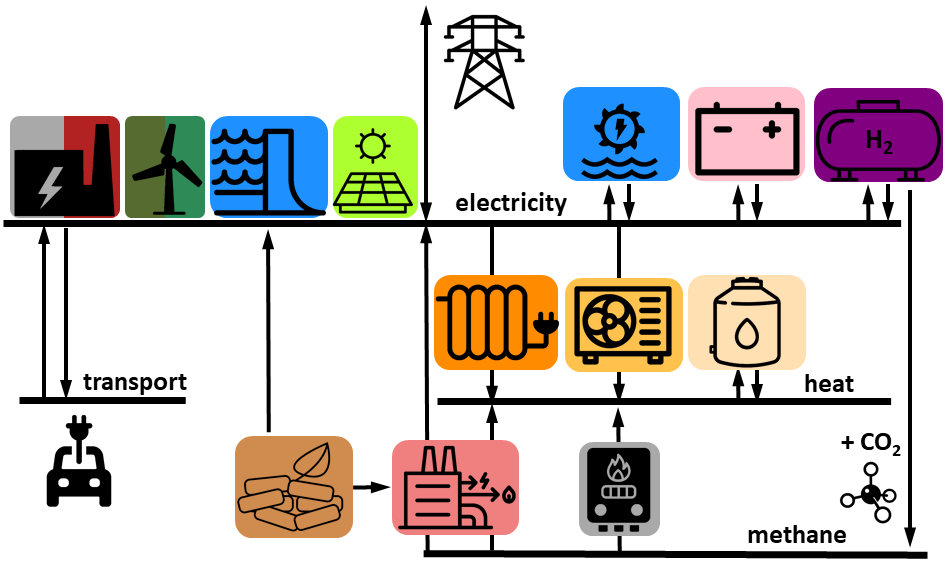
\includegraphics[width=\columnwidth]{figures/model.png}
\caption{Model diagram representing the main technologies and links in every country.} \label{fig_model} 
\end{figure}

\FloatBarrier

\section{Data availability and code availability}

The model is implemented in the open-source framework Python for Power System Analysis (PyPSA) \cite{PyPSA}. The model and data used in this paper can be retrieved from \textcolor[rgb]{1,0,0}{XXX}

\section{Authors contribution}

M. Victoria designed the analysis, drafted the manuscript and contributed to the data acquisition, analysis and interpretation of data. K. Zhu contributed to the data acquisition, modelling, analysis and interpretation of data. 
T. Brown, G. B. Andresen and M. Greiner made substantial revisions of the manuscript. 

\section{Acknowledgements}
M. Victoria, K. Zhu, G. B. Andresen and M. Greiner are fully or partially funded by the RE-INVEST project, which is supported by  the  Innovation  Fund  Denmark  under  grant  number  6154-00022B. T.B. acknowledges funding from the Helmholtz Association under grant no. VH-NG-1352. The responsibility for the contents lies solely with the authors.

\section{References}
\bibliography{bib_transition}

\end{document}